
This section does not really describe a single experiment, and could actually be expanded to cover a whole new thesis.
The study of the optimal pulse shapes (for the drive/control pulse in particular) is one of the most active research topics in the quantum control field.
It is important to understand that this section just provides an example.

To introduce the DRAG~\cite{Gambetta2011} (Derivative Removal by Adiabatic Gate) technique we can start remembering that a superconducting qubit is just an approximation of a two-level system.
Moreover, the difference in frequency between the transition 0-1 and 1-2 is not even particularly large.
The DRAG is the analytical solution to force the interaction Hamiltonian expressed in \cref{eq:drive_hamiltonian} to be restricted to the computational space defined as the state 0-1.

From the theory point of view, we can solve for $A(t)$:
\begin{equation}
    H_{I\;eff}(t) - A^\dagger (t) H (t) A (t) + i \dot{A}^\dagger (t) A (t)
\end{equation}

Leaving to more reliable sources~\cite{Motzoi2009} the burden of the proof, this translates in a modification of our Gaussian pulses, with the addition of a derivative term:
\begin{align}
    i &= Gaussian(x,amp,sigma) = amp * e^{-\frac{1}{2}\left( \frac{x-duration/2}{sigma}\right)^2}\\
    q &= -1j * \beta \left( \frac{x - duration/2}{\sigma^2} \right) * Gaussian
\end{align}

From the shape point of view of the shape this produces an effect visible in \cref{fig:drag_shape}.
\begin{figure}[ht]
    \centering
    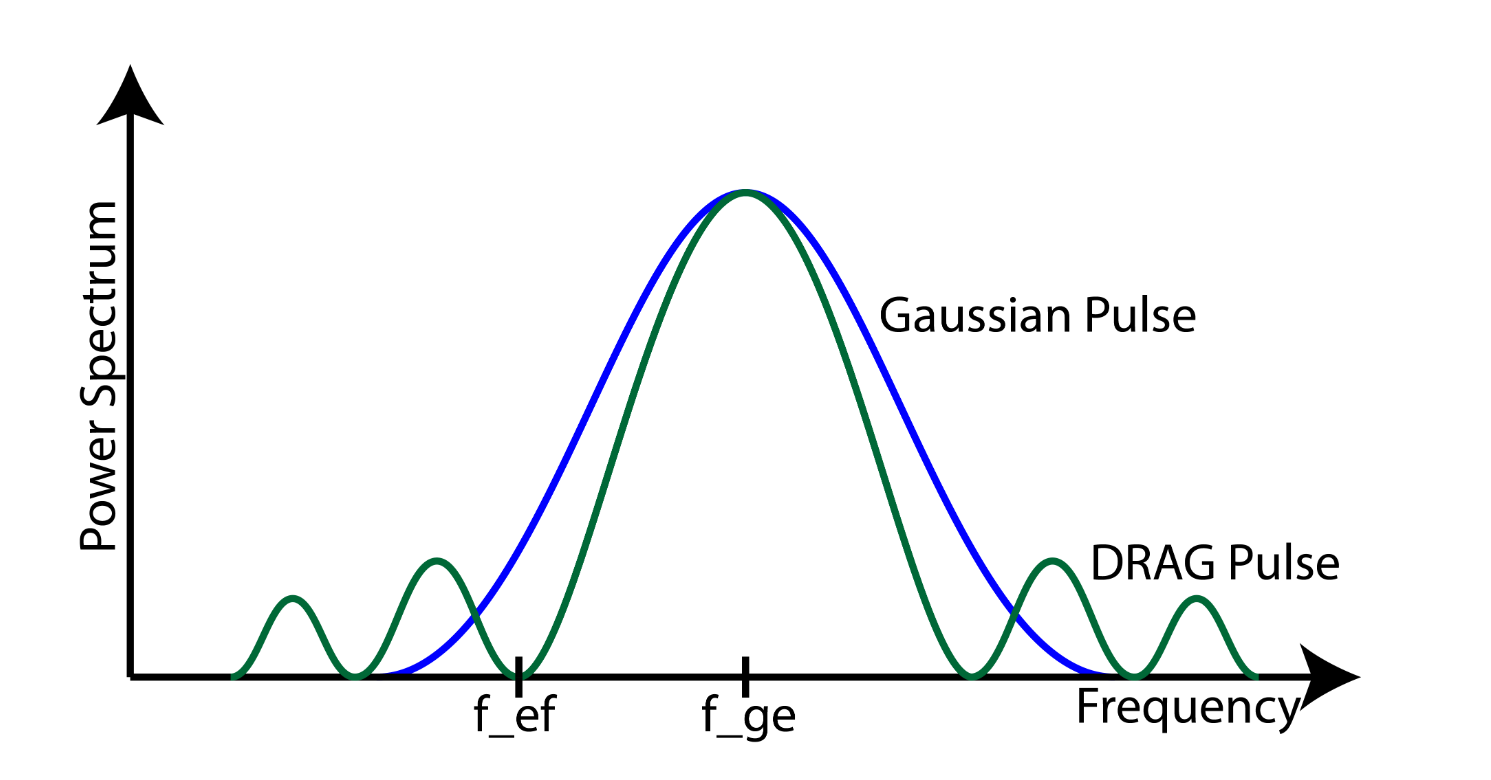
\includegraphics[width=8cm]{characterization/figures/DRAG_gaus.png}
    \caption{Comparison between a Gaussian and a DRAG shapes~\cite{Balasiu2017}.}
    \label{fig:drag_shape}
\end{figure}

From another point of view, we can consider the DRAG pulse as a Gaussian pulse to which it got removed the 1-2 transition frequency $\Delta_{12}$.
In fact we have that the $\beta$ parameter, that is a free, to-be-calibrated parameter is of the magnitude order of $1/\Delta_{12}$.

The calibration of $\beta$ is rather empirical and consists in just repeating the allXY experiment for different hypothesis of $\beta$.\\
Moreover, it is important to note that pulse shape optimization usually does not lead to extremely better results, although it can slightly improve performances.

\experimentrecap
{Drag tuning}
{drive pulse optimization}
{DRAG parameter $\beta$}
{the allXY experiment is repeated for different values of $\beta$. The value that minimizes the distance between the measured points and the expected ones is selected as the calibrated $\beta$.}



